\chapter{Reducing the computational cost}
\label{ch:reducing}

\begin{itemize}
	\item As mentioned in section , evaluating the objective function needs computing all the pairwise distances between the points. Also, the evaluating the gradient is expensive. This is done in $\mathcal{O}(N^2D^2)$ flops. So it is not trivial to successfully use NCA on large data sets.
	\item This chapter presents a wide palette of ideas and methods that can be applied to speed up the computations. Most of the methods rely on the fact that the learnt metric is low ranked.
	\item Every method presented can be regarded as an alteration of the original objective function. We basically change our objective function such that the new objective will have a reduced cost.
\end{itemize}

\section{Sub-sampling}
\label{sec:sub-sampling}

Sub-sampling is the simplest idea that can help speeding up the computations. For the training procedure we use a randomly selected sub-set $\mathcal{D}_n$ of the original data set $\mathcal{D}$:
 \[
 	\mathcal{D}_n = \{ \xB_{i_1},\cdots,\xB_{i_n} \} \subseteq \mathcal{D}.
 \]
 If $n$ is the size of the sub-set then the cost of the gradient is reduced to $\mathcal{O}(n^2D^2)$. After the projection matrix $\AB$ is learnt, it can be applied to the whole data set and all the data points are used for classification.

While easy to implement, this method discards a lot of information available. Also it is affected by the fact the sub-sampled data has a thinner distribution than the real data. 

\begin{figure}
  \centering
  \subfigure[Learnt projection $\AB$ on the sub-sampled data set $\mathcal{D}_n$.]{\label{fig:sub-sampling-1}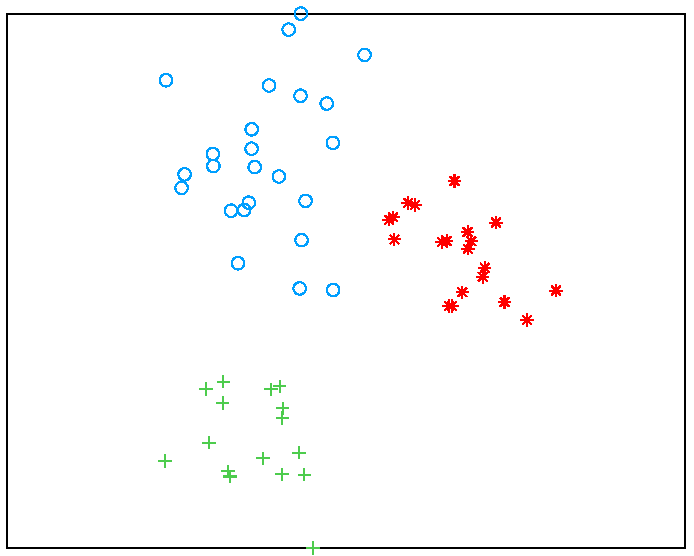
\includegraphics[width=0.48\textwidth]{images/sub-sample-1}}
\subfigure[The projection $\AB$ applied to the whole data set $\mathcal{D}$.]{\label{fig:sub-sampling-2}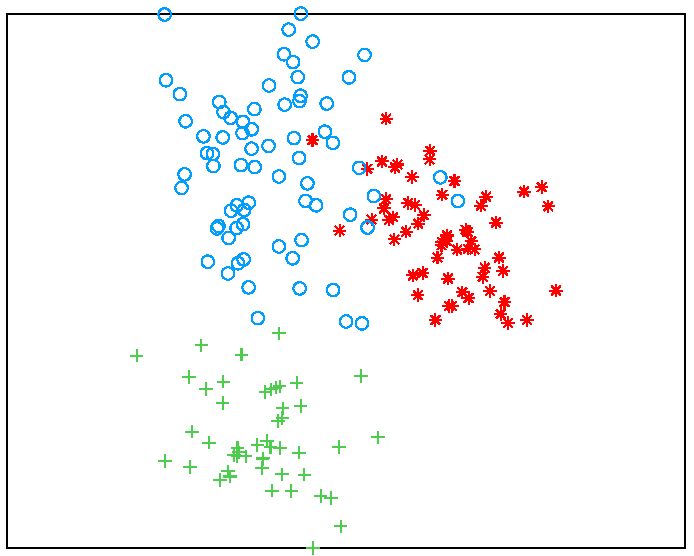
\includegraphics[width=0.48\textwidth]{images/sub-sample-2}}
  \caption{Result of sub-sampling method on \texttt{wine}. There were used one third of the original data set for training, \textit{i.e.}, $n = N/3$. We note that the points that belong to the sub-set $\mathcal{D}_n$ are perfectly separated. But after applying the metric to the whole data there appear different misclassifications. The effects are even more acute if we use smaller sub-sets.}
  \label{fig:sub-sampling}
\end{figure}

\section{Mini-batches}
\label{sec:mini-batches}

The next obvious idea is to use sub-sets in an iterative manner, similar to the stochastic gradient descent method: split the data into mini-batches and train on them successively. Again the cost for one evaluation of the gradient will be $\mathcal{O}(n^2D^2)$ if the mini-batch consists of $n$ points.

\begin{algorithm} 
	\caption{Training algorithm using mini-batches formed by clustering} 
	\label{alg:mini-batches}  
	\begin{algorithmic} [1]                 % enter the algorithmic environment
		\REQUIRE Data set $\mathcal{D}=\{\xB_1,\cdots,\xB_N\}$ and initial linear transformation $\AB$.
		\REPEAT
			\STATE Project each data point using $\AB$:  $\mathcal{D}_\AB=\{\AB\xB_1,\cdots,\AB\xB_N\}$.
			\STATE Use either algorithm \ref{alg:fpc} or \ref{alg:rpc} on $\mathcal{D}_\AB$ to split $\mathcal{D}$  into $K$ mini-batches $\mathcal{M}_1,\cdots,\mathcal{M}_K$.
			\FORALL {$\mathcal{M}_i$}
				\STATE {Update parameter: $\AB\leftarrow \AB - \eta\frac{\partial f(\AB,\mathcal{M}_i)}{\partial\AB}$.}
				\STATE {Update learning rate $\eta$.}
			\ENDFOR
		\UNTIL {convergence.}
	\end{algorithmic}
\end{algorithm}

There are different possibilities for splitting the data-set:
\begin{enumerate}
	\item Random selection. In this case the points are assigned randomly to each mini-batch and after one pass through the whole data set another random allocation is done. As in section \ref{sec:sub-sampling}, this suffers from the thin distribution problem. In order to alleviate this and achieve convergence, large-sized mini-batches should be used (similar to Laurens van der Maaten's implementation). The algorithm is similar to Algorithm \ref{alg:mini-batches}, but lines 2 and 3 will be replaced with a simple random selection.
	
	\item Clustering. Constructing mini-batches by clustering ensures that the point density in each mini-batch is conserved. In order to maintain a low computational cost, we consider cheap clustering methods, \textit{e.g.}, farthest point clustering (FPC; \citealp{gonzalez1985}) and recursive projection clustering (RPC; \citealp{chalupka2011}). Algorithm 
	
	FPC gradually selects cluster centres until it reaches the desired number of clusters $K$. The point which is the farthest away from all the current centres is selected as new centre. The precise algorithm is presented below.
	
	\begin{algorithm} 
		\caption{Farthest point clustering} 
		\label{alg:fpc}  
		\begin{algorithmic}                    % enter the algorithmic environment
			\REQUIRE Data set $\mathcal{D}=\{\xB_1,\cdots,\xB_N\}$ and $K$ number of clusters.
			\STATE Randomly pick a point that will be the first centre $\cB_1$.
			\STATE Allocate all the points in the first cluster $\mathcal{M}_1 \leftarrow \mathcal{D}$.
			\FOR {$i=1$ to $K$}
				\STATE Select the $i$-th cluster centre $\cB_i$ as the point that is farthest away from any cluster centre $\cB_1,\cdots,\cB_{i-1}$.
				\STATE Move to the cluster $\mathcal{M}_i$ those points that are closer to its centre than to any other cluster centre: $\mathcal{M}_i = \left\{ \xB \in \mathcal{D} \;| \; d(\xB;\cB_i) < d(\xB;\cB_j), \forall j \neq i \right\}$
			\ENDFOR
		\end{algorithmic}
	\end{algorithm}
	
	This computational cost of this method is $\mathcal{O}(NK)$. However, we do not have any control on the number of points in each cluster, so we might end up with very unbalanced clusters. A very uneven split has a couple of obvious drawbacks: too large mini-batches will maintain high cost, while on too small clusters there is not too much too learn.
	
	So, as an alternative, RPC was especially developed to mitigate this problem. It constructs the clusters similarly to how the $k$-d trees are build (see section ). However instead of splitting the data set across axis aligned direction it chooses the splitting directions randomly (see algorithm \ref{alg:rpc}). So, because it uses the median value it will result in similar sized clusters and we can easily control the dimension of each cluster. The complexity of this algorithm is $\mathcal{O}()$.
	
	\begin{algorithm} 
		\caption{Recursive projection clustering} 
		\label{alg:rpc}  
		\begin{algorithmic}                    % enter the algorithmic environment
			\REQUIRE Data set $\mathcal{D}=\{\xB_1,\cdots,\xB_N\}$ and $n$ size of clusters.
			\IF {$n < N$}
				\STATE New cluster: $i\leftarrow i+1$.
				\RETURN current points as a cluster: $\mathcal{M}_i \leftarrow \mathcal{D}$.
			\ELSE
				\STATE {Randomly select two points $\xB_j$ and $\xB_k$ from $\mathcal{D}$.}
				\STATE {Project all data points onto the line defined by $\xB_j$ and $\xB_k$. (Give equation?)}
				\STATE {Select the median value $\tilde{\xB}$ from the projected points.}
				\STATE {Recurse on the data points above and below $\tilde{\xB}$: $\text{RPC}(\mathcal{D}_{>\tilde{\xB}})$ and $\text{RPC}(\mathcal{D}_{\le\tilde{\xB}})$.}
%							$\mathcal{D}_{>\tilde{\xB}}=\{\xB\in\mathcal{D}|\xB>\tilde{\xB}\}$
			\ENDIF
		\end{algorithmic}
	\end{algorithm}
	
	Note that we are re-clustering in the transformed space after one sweep through the whole data set. There are also other alternatives. For example, we could cluster in the original space periodically or we could cluster only once in the original space. However the proposed variant has the advantage of a good behaviour for a low rank projection matrix $\AB$. Not only that is cheaper, but the clusters resulted in low dimensions by using RPC are closer to the real clusters then applying the same method in a high dimensional space. 
	
	Further notes:
	\begin{itemize}
		\item The learning rate can be updated using various heuristics as presented in the section related to optimization.
		\item The convergence can be tested in various ways: stop when there is not enough momentum in the parameter space, when the function value doesn't vary too much or by using early stopping or a maximum number of iterations. Discuss all of these in practical issues section.
	\end{itemize}
	
\end{enumerate}

%\begin{center}
%	\begin{table}
%		\centering
%		\begin{tabular}{l}
%			\toprule
%			Training algorithm using mini-batches\\
%			\midrule
%			\textbf{Do}\\
%			Split data $\mathcal{D}$ into mini-batches: $\mathcal{M}_1,\cdots,\mathcal{M}_m$,\\
%			such that $\mathcal{M}_1\cup\cdots\cup\mathcal{M}_m=\mathcal{D}$\\
%			\textbf{For each} mini-batch $\mathcal{M}_i$\\
%			$\AB\leftarrow \AB - \eta\frac{\partial f(\AB,\mathcal{M}_i)}{\partial\AB}$\\
%			\textbf{End for}\\
%			\textbf{Until} we reach convergence\\
%			\bottomrule
%		\end{tabular}
%		\caption{Algorithm for training with mini-batches. The learning is done using gradeint ascent.}
%	\end{table}
%\end{center}


\section{Stochastic learning}
\label{sec:stochastic-learning}


\section{Approximate computations}
\label{sec:approximate}


\section{Exact computations}
\label{sec:exact-computations}

The counterpart of the approximate methods are the exact computations. These are also obtained at some cost. We have to change our model such that it allows efficient exact methods. Again motivated by the rapid decaying squared exponential function, some of the contributions are almost zero. The idea is just to use a compact support kernel instead of the squared exponential kernel. After this is done, there will be a large number of points that will lie outside the support of the kernel and their contribution will be exactly zero instead of a very small value in the previous case.

The kernel needs to be differentiable, so we will use the simplest polynomial compact support kernel that satisfies this requirement. Of course, any other kernel that satisfies this two requirements can be used. This is given by the following expression:
\begin{align}
	k(u)=\begin{cases}
		\frac{15}{16}(a^2-u^2)^2& \mbox{if } u \in [-a;+a]\\
		0& \mbox{otherwise}.\\
	\end{cases}
	\label{eq:cs-1}
\end{align}
The expression from equation \ref{eq:cs-1} also integrates to one, so it can be used in the kernel density estimation context: $p(\xB_i|\xB_j) = k(d(\xB_i;\xB_j))$. 

For the simple replacement of the exponential kernel, we have preferred a simplified version of equation \ref{eq:cs-1}: 
	\begin{align}
		k(u)=\begin{cases}
				(1-u^2)^2& \mbox{if } u \in [-1;1]\\
				0& \mbox{otherwise}.\\
			\end{cases}
			\label{eq:cs-2}
	\end{align}
	
	The width of the kernel's support $a$ will be integrated in the projection matrix $\AB$, similarly as the widths for the Gaussian kernel are absorbed by $\AB$ for the classic NCA.

\begin{align}
	p_{ij} = \frac{k(d_{ij})}{\sum_{k\neq i} k(d_{ik})}.
\end{align}

Objective function will be: 
\begin{align}
	f_\text{CS}(\AB) = \sum_{i}\sum_{j\in c_i} p_{ij}
\end{align}

The gradient of the kernel:
\begin{align}
	\frac{\partial}{\partial\AB}k(d_{ij}) 
	&= 	\frac{\partial}{\partial\AB}\left[(1-d_{ij}^2)^2\cdot\mathrm{I}(\left|d_{ij}\right|\le 1)\right]\\
	&= -4\AB(1-d_{ij}^2)  \xB_{ij} \xB_{ij}^\mathrm{T} \cdot \mathrm{I}(\left|d_{ij}\right|\le 1),
\end{align}
where $d_{ij}^2 = d(\AB\xB_i;\AB\xB_j)$, $\xB_{ij}=\xB_i-\xB_j$ and $\mathrm{I}(\cdot)$ is the indicator function that return 1 when its argument is true and 0 when its argument is false.

The gradient of the new objective function:
\begin{align}
	\frac{\partial f_\text{CS}}{\partial \AB}=2\AB\sum_{i=1}^{N}
	\left(
	p_i \sum_{k=1}^N \frac{p_{ik}}{1-d_{ik}^2} \xB_{ik}\xB_{ik}^{\textrm{T}}
	- \sum_{j\in c_i} \frac{p_{ij}}{1-d_{ij}^2}\xB_{ij}\xB_{ij}^{\textrm{T}} 
	\right)
	\label{eq:nca-cs-grad},
\end{align}

The main concern with this method is what happens when points lie outside the compact support of any other point in the data set. So care must be taken at initialisation. One way would be to initialise with a very small scale $\AB$. However, this means that there is no gain in speed for at least the first iterations. It might be better to use the principal components for initialisation. 

\begin{itemize}
	\item Speedings comes from the fact only few gradient components need to be computed. A nice way of further accelerating this is again via $k$-d trees. This time they can be used for range search. 
	\item Note regarding the gradient: it was written in this form for simplicity. However, in an implementation it is not recommended to divide each term by $1-d_{ij}^2$; there might results cases that are not determined. Better is to compute the kernel values in two steps.
\end{itemize}

\section{NCA with compact support kernels and background distribution}
\label{sec:nca-cs-back}


\begin{figure}
  \centering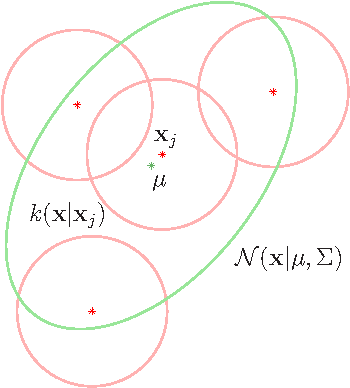
\includegraphics[width=6cm]{images/nca-cs-back}
  \caption{Neighbourhood component analysis with compact support kernels and background distribution. Main assumption: each class is class is a mixture of compact support distributions $k(\xB|\xB_j)$ plus the normal background distribution $\mathcal{N}(\xB|\muB,\SigmaB)$.}
  \label{fig:cs-back}
\end{figure}

\begin{itemize}
	\item An extended variant of the previous scenario. We take care of the points that might remain unallocated by using a background distribution. This extension comes on naturally after the CC-KDE formulation. We can change the assumptions regarding the underlying distribution of a class $p(\xB_i|c)$. So, in this case, we consider that a point can be generated from a class by either a compact distribution from each point $k_\text{CS}(\xB_i|\xB_j)$ or by a global normal distribution that is specific to the whole class $\mathcal{N}(\xB_i|\muB_c,\SigmaB_c)$. So, the class-conditional distribution is given by the sum of these components:
	\begin{align}
		p(\xB_i|c) = \beta \mathcal{N}(\xB_i|\muB_c,\SigmaB_c) + (1-\beta) \frac{1}{N_c}\sum_{j\in c} k_\text{CS}(\xB_i|\xB_j),
		\label{eq:nca-cs-back-1}
	\end{align}
	where $\beta$ is the mixing coefficient between the background distribution and the compact support model and $\muB_c$ and $\SigmaB_c$ are the sample mean and covariance of the class $c$.
	\item It is unclear how we can choose the mixing proportion $\beta$. By setting $\beta = \frac{1}{N_c+1}$ we will give equal weights to the background distribution as to the compact-support distribution. Setting it too large means that the model will favour convex classes. On one hand, this might diminish NCA's power. One of its strengths lies in the ability to work on non-convex classes. On the other hand, some of the classes  This can be fitted as a parameter during the optimization process. The gradient with respect to $\beta$ can be easily derived and it is easy to evaluate it as the quantities required for this should also be computed for the function evaluation. 
	\item This model can be used by plugging equation \ref{eq:nca-cs-back-1} into the set of equations \ref{eq:nca-cc-kde-bayes}, \ref{eq:nca-cc-kde-obj} and \ref{eq:nca-cc-kde-grad} from section \ref{sec:cc-kde}. 
	\item We give here the gradient for the background distribution with respect to the point positions (the full derivation can be found in the appendix). 
	\item It might be useful to note that projecting the points $\{\xB_i\}_{i=1}^N$ into a new space $\{\AB\xB_i\}_{i=1}^N$ will change the sample mean $\muB_c$ to $\AB\muB_c$ and the sample covariance $\SigmaB_c$ to $\AB\SigmaB_c\AB^\mathrm{T}$. Hence, we have:
	\begin{align}
		\frac{\partial}{\partial \AB} \mathcal{N}(\AB\xB_i&|\AB\muB_c, \AB\SigmaB_c \AB^\mathrm{T}) = \mathcal{N}(\AB\xB_i|\AB\muB_c, \AB\SigmaB_c \AB^\mathrm{T})\notag\\
		&\times \{ -(\AB\SigmaB_c \AB^\mathrm{T})^{-1}\AB\SigmaB_c
		+\vB \vB ^ \mathrm{T} \AB \SigmaB_c - \vB (\xB - \muB_c)^\mathrm{T}
		\},
	\end{align}
	where $\vB = (\AB\SigmaB_c \AB^\mathrm{T})^{-1}\AB(\xB - \muB_c)$.
\end{itemize}
